% Standalone TikZ figure: Reward Shaping Illustration
% For Chapter 7: Reward Function Engineering
\documentclass[tikz,border=10pt]{standalone}
\usepackage{tikz}
\usepackage{amsmath}
\usetikzlibrary{arrows.meta, positioning, shapes.geometric, calc, patterns, decorations.pathreplacing}

\begin{document}
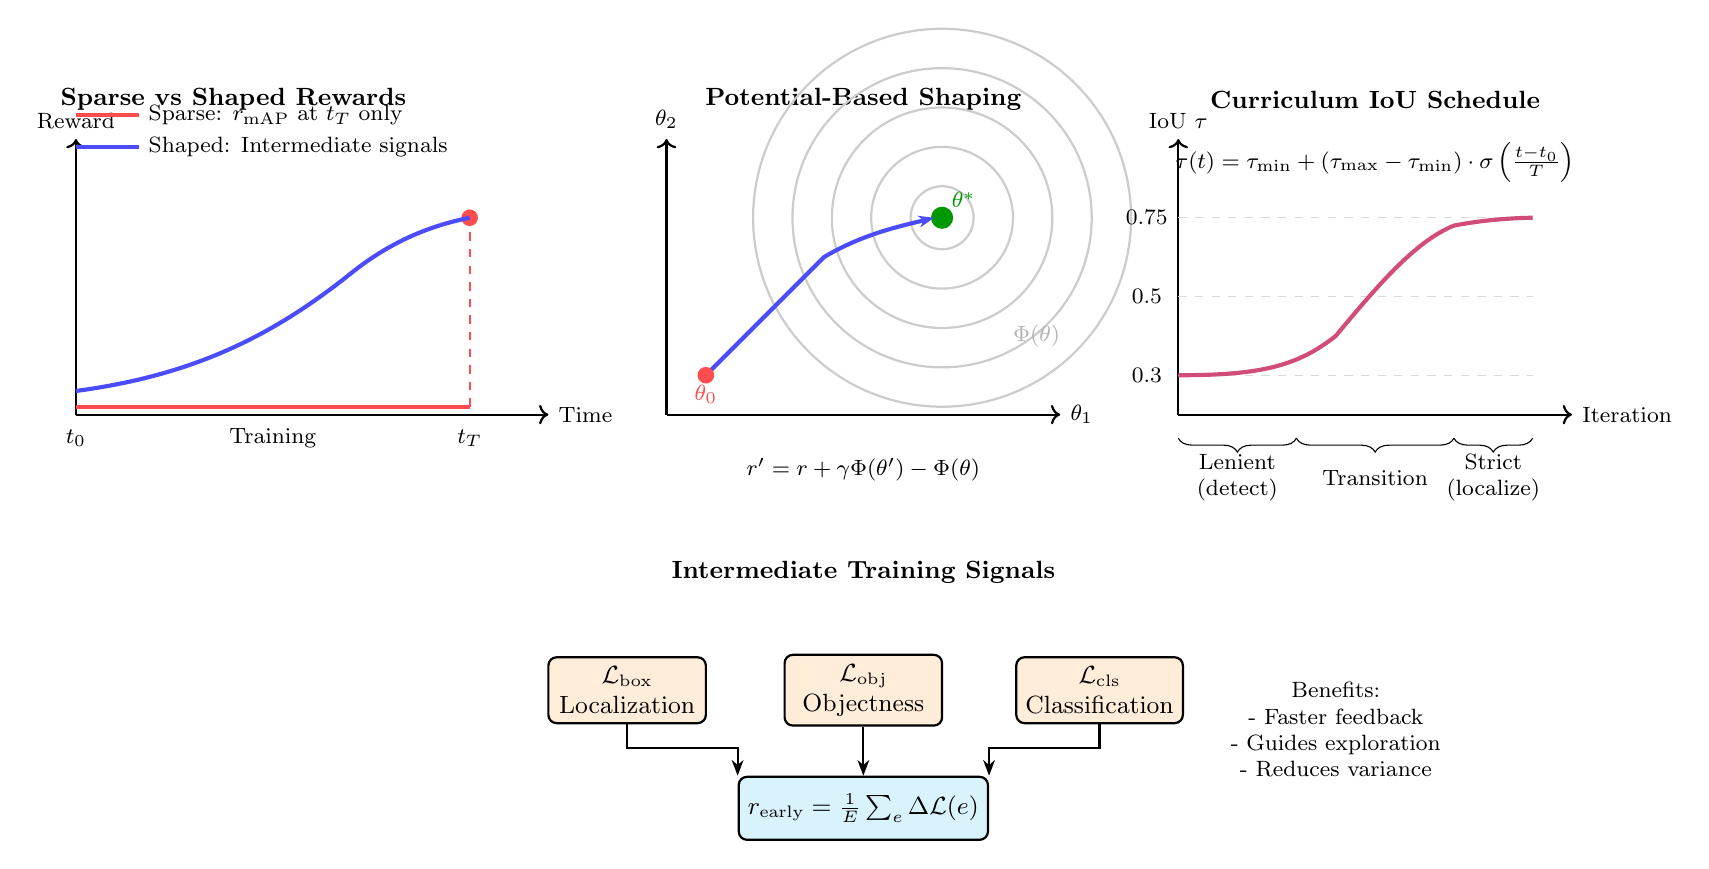
\begin{tikzpicture}[
    node distance=1.2cm and 1.5cm,
    every node/.style={font=\small},
    box/.style={rectangle, draw, thick, minimum width=2cm, minimum height=0.8cm, align=center, rounded corners=3pt},
    arrow/.style={-{Stealth[length=2mm]}, thick},
    label/.style={font=\footnotesize},
    title/.style={font=\bfseries\small}
]

% ============ SPARSE vs SHAPED REWARDS (LEFT) ============
\node[title] at (0, 4) {Sparse vs Shaped Rewards};

% Timeline axis
\draw[thick, ->] (-2, 0) -- (4, 0) node[right, label] {Time};
\draw[thick, ->] (-2, 0) -- (-2, 3.5) node[above, label] {Reward};

% Sparse reward (only at end)
\draw[thick, red!70, line width=1.5pt] (-2, 0.1) -- (2.8, 0.1);
\fill[red!70] (3, 2.5) circle (3pt);
\draw[thick, red!70, line width=1.5pt] (2.8, 0.1) -- (3, 0.1);
\draw[thick, red!70, dashed] (3, 0.1) -- (3, 2.5);

% Shaped reward (progressive)
\draw[thick, blue!70, line width=1.5pt]
    (-2, 0.3) .. controls (-0.5, 0.5) and (0.5, 1) .. (1.5, 1.8) .. controls (2, 2.2) and (2.5, 2.4) .. (3, 2.5);

% Time markers
\node[label] at (-2, -0.3) {$t_0$};
\node[label] at (0.5, -0.3) {Training};
\node[label] at (3, -0.3) {$t_T$};

% Legend
\draw[thick, red!70, line width=1.5pt] (-2, 3.8) -- (-1.2, 3.8);
\node[label, right] at (-1.2, 3.8) {Sparse: $r_{\text{mAP}}$ at $t_T$ only};
\draw[thick, blue!70, line width=1.5pt] (-2, 3.4) -- (-1.2, 3.4);
\node[label, right] at (-1.2, 3.4) {Shaped: Intermediate signals};

% ============ POTENTIAL-BASED SHAPING (CENTER) ============
\node[title] at (8, 4) {Potential-Based Shaping};

% State space with potential function contours
\draw[thick, ->] (5.5, 0) -- (10.5, 0) node[right, label] {$\theta_1$};
\draw[thick, ->] (5.5, 0) -- (5.5, 3.5) node[above, label] {$\theta_2$};

% Potential contours (concentric toward goal)
\draw[gray!40, thick] (9, 2.5) circle (0.4);
\draw[gray!40, thick] (9, 2.5) circle (0.9);
\draw[gray!40, thick] (9, 2.5) circle (1.4);
\draw[gray!40, thick] (9, 2.5) circle (1.9);
\draw[gray!40, thick] (9, 2.5) circle (2.4);

% Good configuration (goal)
\fill[green!60!black] (9, 2.5) circle (4pt);
\node[label, green!60!black, above right] at (9, 2.5) {$\theta^*$};

% Trajectory with shaping
\draw[thick, blue!70, -{Stealth[length=2mm]}, line width=1.5pt]
    (6, 0.5) .. controls (6.5, 1) and (7, 1.5) .. (7.5, 2) .. controls (8, 2.3) and (8.5, 2.4) .. (8.9, 2.5);

% Start point
\fill[red!70] (6, 0.5) circle (3pt);
\node[label, red!70, below] at (6, 0.5) {$\theta_0$};

% Potential values
\node[label, gray!60] at (10.2, 1) {$\Phi(\theta)$};
\node[label, align=center] at (8, -0.7) {$r' = r + \gamma\Phi(\theta') - \Phi(\theta)$};

% ============ CURRICULUM SCHEDULE (RIGHT) ============
\node[title] at (14.5, 4) {Curriculum IoU Schedule};

% Axes
\draw[thick, ->] (12, 0) -- (17, 0) node[right, label] {Iteration};
\draw[thick, ->] (12, 0) -- (12, 3.5) node[above, label] {IoU $\tau$};

% Y-axis labels
\node[label] at (11.6, 0.5) {0.3};
\node[label] at (11.6, 1.5) {0.5};
\node[label] at (11.6, 2.5) {0.75};

% Horizontal reference lines
\draw[gray!30, dashed] (12, 0.5) -- (16.5, 0.5);
\draw[gray!30, dashed] (12, 1.5) -- (16.5, 1.5);
\draw[gray!30, dashed] (12, 2.5) -- (16.5, 2.5);

% Sigmoid curriculum schedule
\draw[thick, purple!70, line width=1.5pt]
    (12, 0.5) .. controls (13, 0.5) and (13.5, 0.6) .. (14, 1) .. controls (14.5, 1.6) and (15, 2.2) .. (15.5, 2.4) .. controls (16, 2.5) and (16.5, 2.5) .. (16.5, 2.5);

% Phase annotations
\draw[decorate, decoration={brace, amplitude=5pt, mirror}] (12, -0.3) -- (13.5, -0.3);
\node[label, align=center] at (12.75, -0.8) {Lenient\\(detect)};

\draw[decorate, decoration={brace, amplitude=5pt, mirror}] (13.5, -0.3) -- (15.5, -0.3);
\node[label, align=center] at (14.5, -0.8) {Transition};

\draw[decorate, decoration={brace, amplitude=5pt, mirror}] (15.5, -0.3) -- (16.5, -0.3);
\node[label, align=center] at (16, -0.8) {Strict\\(localize)};

% Formula
\node[align=center, label] at (14.5, 3.2) {$\tau(t) = \tau_{\min} + (\tau_{\max} - \tau_{\min}) \cdot \sigma\left(\frac{t - t_0}{T}\right)$};

% ============ INTERMEDIATE REWARDS (BOTTOM) ============
\node[title] at (8, -2) {Intermediate Training Signals};

% Loss curve boxes
\node[box, fill=orange!15] (loss1) at (5, -3.5) {$\mathcal{L}_{\text{box}}$\\Localization};
\node[box, fill=orange!15] (loss2) at (8, -3.5) {$\mathcal{L}_{\text{obj}}$\\Objectness};
\node[box, fill=orange!15] (loss3) at (11, -3.5) {$\mathcal{L}_{\text{cls}}$\\Classification};

% Aggregation
\node[box, fill=cyan!15, minimum width=3cm] (inter) at (8, -5) {$r_{\text{early}} = \frac{1}{E}\sum_e \Delta\mathcal{L}(e)$};

% Arrows
\draw[arrow] (loss1.south) -- ++(0,-0.3) -| (inter.north west);
\draw[arrow] (loss2.south) -- (inter.north);
\draw[arrow] (loss3.south) -- ++(0,-0.3) -| (inter.north east);

% Benefit annotation
\node[label, align=center] at (14, -4) {Benefits:\\- Faster feedback\\- Guides exploration\\- Reduces variance};

\end{tikzpicture}
\end{document}
